\documentclass[11pt]{article}
\usepackage{amsmath}
\usepackage{amssymb} 
\usepackage{tikz}
\usepackage{geometry}
\usepackage{xcolor}
\usepackage[most]{tcolorbox} % 'most' is required for the breakable option
\geometry{a4paper, margin=1in}
\usepackage{cancel}

% --- Custom Colors ---
\definecolor{mainblue}{RGB}{0, 102, 204}
\definecolor{trapred}{RGB}{204, 0, 0}
\definecolor{conceptgreen}{RGB}{0, 153, 76}

% --- Custom Box Environments ---
\newtcolorbox{stepbox}[1][]{
    colback=mainblue!5!white,
    colframe=mainblue,
    fonttitle=\bfseries,
    title={#1}, % <--- ADDED CURLY BRACES HERE
    arc=2mm,
    boxrule=1pt,
    breakable 
}

\newtcolorbox{conceptbox}[1][]{
    colback=conceptgreen!5!white,
    colframe=conceptgreen,
    fonttitle=\bfseries,
    title={#1}, % <--- ADDED CURLY BRACES HERE
    arc=2mm,
    boxrule=1pt,
    breakable
}


\newtcolorbox{examtrap}[1][]{
    colback=trapred!5!white,
    colframe=trapred,
    fonttitle=\bfseries,
    title=#1,
    arc=2mm,
    boxrule=1pt,
    breakable
}

\begin{document}

\title{\textbf{Power Systems: The Ultimate Newton-Raphson Load Flow Guide}}
\author{Mubarok Hossen Kamil}
\date{}
\maketitle

% ==========================================
% THEORY SECTION
% ==========================================
\section*{\textcolor{mainblue}{Theory: The Newton-Raphson Method}}

While the Gauss-Seidel method is simple, it requires dozens (sometimes hundreds) of iterations to solve large power grids. The \textbf{Newton-Raphson (N-R) method} uses Calculus to calculate exact slopes (derivatives), allowing it to solve systems of any size in usually 3 to 5 iterations.

\subsection*{1. The General Power Flow Equations}
The active ($P$) and reactive ($Q$) power injected at any bus $i$ is calculated as:
\begin{align}
    P_i &= \sum_{n=1}^{N} |V_i V_n Y_{in}| \cos(\theta_{in} + \delta_n - \delta_i) \label{eq:P_theory} \\
    Q_i &= -\sum_{n=1}^{N} |V_i V_n Y_{in}| \sin(\theta_{in} + \delta_n - \delta_i) \label{eq:Q_theory}
\end{align}

\subsection*{2. Power Mismatches}
At each iteration, we compare our \textit{calculated} power (using our guessed voltages) with the \textit{scheduled} (actual physical) power to find the mismatch ($\Delta$):
\begin{align*}
    \Delta P_i &= P_i^{sch} - P_i^{calc} \\
    \Delta Q_i &= Q_i^{sch} - Q_i^{calc}
\end{align*}


\subsection*{3. How to Build the $Y_{bus}$ Matrix}

If the power system has $N$ buses, the $Y_{bus}$ is an $N \times N$ grid. There are two simple rules to build it:

\begin{conceptbox}[{Two Simple Rules for $Y_{bus}$}]
\textbf{(i) The Diagonal elements ($Y_{11}, Y_{22}$, etc.)} \\
$\rightarrow$ This is the \textit{self-admittance}. \\
\textbf{Rule:} To find $Y_{ii}$, simply add up the admittances of every single line directly connected to Bus $i$.

\vspace{0.3cm}
\textbf{(ii) The off-diagonal elements ($Y_{12}, Y_{13}, Y_{23}$, etc.)} \\
$\rightarrow$ This is the \textit{mutual admittance} between two buses. \\
\textbf{Rule:} To find $Y_{ij}$, take the admittance of the line connecting Bus $i$ to Bus $j$, and multiply it by $(-1)$. If there is no line connecting them, it's 0.
\end{conceptbox}

\begin{stepbox}[{$Y_{bus}$ Example Calculation}]
Imagine a tiny 3-bus system, with line admittances given as:
\begin{itemize}
    \item Line connecting bus 1 and bus 2 has $y_{12} = -j10$
    \item Line connecting bus 2 and bus 3 has $y_{23} = -j5$
    \item Line connecting bus 1 and bus 3 has $y_{13} = -j8$
\end{itemize}

Let's build the $3 \times 3$ matrix:

\vspace{0.2cm}
\textbf{Step 1: The diagonal (sum of connected lines)}
\begin{align*}
    Y_{11} &= \text{line touching bus 1} = y_{12} + y_{13} = -j10 - j8 = \mathbf{-j18} \\
    Y_{22} &= \text{line touching bus 2} = y_{12} + y_{23} = -j10 - j5 = \mathbf{-j15} \\
    Y_{33} &= \text{line touching bus 3} = y_{13} + y_{23} = -j5 - j8 = \mathbf{-j13}
\end{align*}

\textbf{Step 2: The off-diagonal (neg of the connecting line)}
\begin{align*}
    Y_{12} &= Y_{21} = -(y_{12}) = -(-j10) = \mathbf{j10} \\
    Y_{13} &= Y_{31} = -(y_{13}) = -(-j8) = \mathbf{j8} \\
    Y_{23} &= Y_{32} = -(y_{23}) = -(-j5) = \mathbf{j5}
\end{align*}

\vspace{0.2cm}
\textbf{Final Resulting Matrix:}
\begin{equation*}
    Y_{bus} = 
    \begin{bmatrix}
    -j18 & j10 & j8 \\
    j10 & -j15 & j5 \\
    j8 & j5 & -j13
    \end{bmatrix}
\end{equation*}
\end{stepbox}

\subsection*{4. Extracting $G$ and $B$ from $Y_{bus}$}
\begin{conceptbox}[{Extracting $G$ and $B$ from $Y_{bus}$}]
Every element in the Admittance Matrix ($Y_{bus}$) is a complex number written in rectangular form:
\begin{equation*}
    Y_{ij} = G_{ij} + jB_{ij}
\end{equation*}
To extract the values for our Newton-Raphson formulas:
\begin{itemize}
    \item $\mathbf{G_{ij}}$ (Conductance) is simply the \textbf{Real} part.
    \item $\mathbf{B_{ij}}$ (Susceptance) is the \textbf{Imaginary} part (including the positive/negative sign, but dropping the '$j$').
\end{itemize}
\textit{Example:} If $Y = 26 - j52$, then $G = 26$ and $B = -52$.
\end{conceptbox}

\subsection*{5. The Jacobian Matrix ($J$)}
The N-R method relates these power mismatches to voltage corrections ($\Delta \delta$ and $\Delta |V|$) using a matrix of partial derivatives called the \textbf{Jacobian}. The general equation is:
\begin{equation*}
    \begin{bmatrix} \Delta P \\ \Delta Q \end{bmatrix} = 
    \begin{bmatrix} J_{11} & J_{12} \\ J_{21} & J_{22} \end{bmatrix} 
    \begin{bmatrix} \Delta \delta \\ \Delta |V| \end{bmatrix}
\end{equation*}


% ==========================================
% MATRIX CONDITIONS SECTION
% ==========================================
\newpage
\section*{\textcolor{mainblue}{Matrix Formulation for Different Bus Conditions}}
The size and structure of the Jacobian matrix dynamically change depending on the types of buses present in the power system. To understand this, we divide the Jacobian into four sub-matrices:
\begin{equation*}
    \begin{bmatrix} \Delta P \\ \Delta Q \end{bmatrix} = 
    \begin{bmatrix} J_1 & J_2 \\ J_3 & J_4 \end{bmatrix} 
    \begin{bmatrix} \Delta \delta \\ \Delta |V| \end{bmatrix}
\end{equation*}
Where:
\begin{itemize}
    \item $\mathbf{J_1 = \frac{\partial P}{\partial \delta}}$ : Relates Real Power to Voltage Angles.
    \item $\mathbf{J_2 = \frac{\partial P}{\partial |V|}}$ : Relates Real Power to Voltage Magnitudes.
    \item $\mathbf{J_3 = \frac{\partial Q}{\partial \delta}}$ : Relates Reactive Power to Voltage Angles.
    \item $\mathbf{J_4 = \frac{\partial Q}{\partial |V|}}$ : Relates Reactive Power to Voltage Magnitudes.
\end{itemize}

\hrule
\vspace{0.2cm}
Below are the matrix setups for the three possible system conditions:

\subsection*{(i) Condition 1: System with ONLY Slack and PQ (Load) Buses}
In a system where Bus 1 is the Slack bus and \textit{all} other buses are PQ (Load) buses, both Real ($P$) and Reactive ($Q$) powers are scheduled/known for every bus except the Slack bus.
\begin{stepbox}[ONLY Slack and PQ (Load) Buses]
\begin{equation*}
    \left[ \begin{array}{c} 
    \Delta P_2 \\ \vdots \\ \Delta P_N \\ \hline
    \Delta Q_2 \\ \vdots \\ \Delta Q_N 
    \end{array} \right] 
    = 
    \left[ \begin{array}{ccc | ccc} 
    \frac{\partial P_2}{\partial \delta_2} & \cdots & \frac{\partial P_2}{\partial \delta_N} & \frac{\partial P_2}{\partial |V_2|} & \cdots & \frac{\partial P_2}{\partial |V_N|} \\
    \vdots & \ddots & \vdots & \vdots & \ddots & \vdots \\
    \frac{\partial P_N}{\partial \delta_2} & \cdots & \frac{\partial P_N}{\partial \delta_N} & \frac{\partial P_N}{\partial |V_2|} & \cdots & \frac{\partial P_N}{\partial |V_N|} \\ \hline
    \frac{\partial Q_2}{\partial \delta_2} & \cdots & \frac{\partial Q_2}{\partial \delta_N} & \frac{\partial Q_2}{\partial |V_2|} & \cdots & \frac{\partial Q_2}{\partial |V_N|} \\
    \vdots & \ddots & \vdots & \vdots & \ddots & \vdots \\
    \frac{\partial Q_N}{\partial \delta_2} & \cdots & \frac{\partial Q_N}{\partial \delta_N} & \frac{\partial Q_N}{\partial |V_2|} & \cdots & \frac{\partial Q_N}{\partial |V_N|}
    \end{array} \right]
    \left[ \begin{array}{c} 
    \Delta \delta_2 \\ \vdots \\ \Delta \delta_N \\ \hline
    \Delta |V_2| \\ \vdots \\ \Delta |V_N|
    \end{array} \right]
\end{equation*}
\end{stepbox}

\vspace{0.5cm}

% --- EXAMPLE 1 ---
\noindent \textbf{\large Example 1: 3-Bus System (1 Slack, 2 PQ Buses)} \\

\begin{center}
\begin{tikzpicture}[>=latex, scale=0.85, transform shape]
    % Bus 1 (Slack)
    \draw[thick, mainblue] (0,4.5) -- (0,1.5);
    \node[above] at (0,4.5) {\textbf{1}};
    \node[left, align=center] at (-1.5,2.5) {Slack Bus\\$|V_1|, \delta_1$};
    \draw (0,3.5) -- (-1,3.5);
    \draw[thick] (-1.4,3.5) circle (0.4) node {$\sim$};

    % Bus 2 (PQ)
    \draw[thick, trapred] (10,4.5) -- (10,1.5);
    \node[above] at (10,4.5) {\textbf{2}};
    \node[above, align=center] at (11.5,4.0) {PQ Bus};
    \draw[->, thick] (10,3.5) -- (11.5,3.5) node[right] {$P_2$ (Load)};
    \draw[->, thick] (10,2.5) -- (11.5,2.5) node[right] {$Q_2$ (Load)};

    % Bus 3 (PQ)
    \draw[thick, conceptgreen] (3.5,0) -- (6.5,0);
    \node[left] at (3.5,0) {\textbf{3}};
    \node[left, align=center] at (2.5,-0.5) {PQ Bus};
    \draw[->, thick] (4.5,0) -- (4.5,-1.5) node[below] {$P_3$ (Load)};
    \draw[->, thick] (5.5,0) -- (5.5,-1.5) node[right] {$Q_3$ (Load)};

    % Lines
    \draw (0,4) -- (10,4) node[midway, above] {Line 1-2};
    \draw (0,2) -- (3,2) -- (3,0);
    \node[above right] at (1.5, 2) {Line 1-3};
    \draw (10,2) -- (7,2) -- (7,0);
    \node[above left] at (8.5, 2) {Line 2-3};
\end{tikzpicture}
\end{center}

\textbf{Matrix Equation for Example 1:}
\begin{equation*}
    \left[ \begin{array}{c} 
    \Delta P_2 \\ \Delta P_3 \\ \hline
    \Delta Q_2 \\ \Delta Q_3
    \end{array} \right] 
    = 
    \left[ \begin{array}{cc | cc} 
    \frac{\partial P_2}{\partial \delta_2} & \frac{\partial P_2}{\partial \delta_3} & \frac{\partial P_2}{\partial |V_2|} & \frac{\partial P_2}{\partial |V_3|} \\[0.3cm]
    \frac{\partial P_3}{\partial \delta_2} & \frac{\partial P_3}{\partial \delta_3} & \frac{\partial P_3}{\partial |V_2|} & \frac{\partial P_3}{\partial |V_3|} \\[0.2cm] \hline \\[-0.3cm]
    \frac{\partial Q_2}{\partial \delta_2} & \frac{\partial Q_2}{\partial \delta_3} & \frac{\partial Q_2}{\partial |V_2|} & \frac{\partial Q_2}{\partial |V_3|} \\[0.3cm]
    \frac{\partial Q_3}{\partial \delta_2} & \frac{\partial Q_3}{\partial \delta_3} & \frac{\partial Q_3}{\partial |V_2|} & \frac{\partial Q_3}{\partial |V_3|}
    \end{array} \right]
    \left[ \begin{array}{c} 
    \Delta \delta_2 \\ \Delta \delta_3 \\ \hline
    \Delta |V_2| \\ \Delta |V_3|
    \end{array} \right]
\end{equation*}

\vspace{0.8cm}

% --- EXAMPLE 2 ---
\noindent \textbf{\large Example 2: 2-Bus System (1 Slack, 1 PQ Bus)} \\
Here, $N = 2$. This is the simplest possible system. We have one Slack bus and one Load (PQ) bus.

\begin{center}
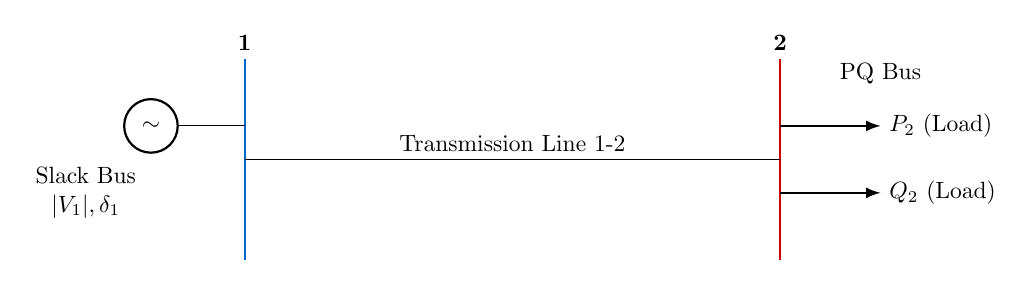
\begin{tikzpicture}[>=latex, scale=0.85, transform shape]
    % Bus 1 (Slack)
    \draw[thick, mainblue] (0,4.5) -- (0,1.5);
    \node[above] at (0,4.5) {\textbf{1}};
    \node[left, align=center] at (-1.5,2.5) {Slack Bus\\$|V_1|, \delta_1$};
    \draw (0,3.5) -- (-1,3.5);
    \draw[thick] (-1.4,3.5) circle (0.4) node {$\sim$};

    % Bus 2 (PQ)
    \draw[thick, trapred] (8,4.5) -- (8,1.5);
    \node[above] at (8,4.5) {\textbf{2}};
    \node[above, align=center] at (9.5,4.0) {PQ Bus};
    \draw[->, thick] (8,3.5) -- (9.5,3.5) node[right] {$P_2$ (Load)};
    \draw[->, thick] (8,2.5) -- (9.5,2.5) node[right] {$Q_2$ (Load)};

    % Line
    \draw (0,3) -- (8,3) node[midway, above] {Transmission Line 1-2};
\end{tikzpicture}
\end{center}

\textbf{Matrix Equation for Example 2:}
\begin{equation*}
    \left[ \begin{array}{c} 
    \Delta P_2 \\ \hline
    \Delta Q_2
    \end{array} \right] 
    = 
    \left[ \begin{array}{c | c} 
    \frac{\partial P_2}{\partial \delta_2} & \frac{\partial P_2}{\partial |V_2|} \\[0.3cm] \hline \\[-0.3cm]
    \frac{\partial Q_2}{\partial \delta_2} & \frac{\partial Q_2}{\partial |V_2|}
    \end{array} \right]
    \left[ \begin{array}{c} 
    \Delta \delta_2 \\ \hline
    \Delta |V_2|
    \end{array} \right]
\end{equation*}

\vspace{0.5cm}
\hrule

\subsection*{(ii) Condition 2: System with Slack, PQ, and PV Buses (Standard Case)}
This is the most common real-world scenario. Assume we have a Slack bus, some PQ (Load) buses, and some PV (Generator) buses. 
For PV buses, the voltage magnitude ($|V|$) is fixed, so $\Delta |V| = 0$, and the reactive power ($Q$) is unknown, meaning we \textbf{cannot write a $\Delta Q$ mismatch equation} for them.
%
\begin{stepbox}[{Slack, PQ, and PV Buses (Standard Case)}]
We remove the $\Delta Q$ rows and $\Delta |V|$ columns corresponding to the PV buses.
\begin{equation*}
    \left[ \begin{array}{c} 
    \Delta P_{PQ} \\ \Delta P_{PV} \\ \hline
    \Delta Q_{PQ} 
    \end{array} \right] 
    = 
    \left[ \begin{array}{cc | c} 
    \frac{\partial P_{PQ}}{\partial \delta_{PQ}} & \frac{\partial P_{PQ}}{\partial \delta_{PV}} & \frac{\partial P_{PQ}}{\partial |V|_{PQ}} \\[0.2cm]
    \frac{\partial P_{PV}}{\partial \delta_{PQ}} & \frac{\partial P_{PV}}{\partial \delta_{PV}} & \frac{\partial P_{PV}}{\partial |V|_{PQ}} \\[0.2cm] \hline
    \frac{\partial Q_{PQ}}{\partial \delta_{PQ}} & \frac{\partial Q_{PQ}}{\partial \delta_{PV}} & \frac{\partial Q_{PQ}}{\partial |V|_{PQ}}
    \end{array} \right]
    \left[ \begin{array}{c} 
    \Delta \delta_{PQ} \\ \Delta \delta_{PV} \\ \hline
    \Delta |V|_{PQ} 
    \end{array} \right]
\end{equation*}
\end{stepbox}

\vspace{0.5cm}

% --- EXAMPLE 1 ---
\noindent \textbf{\large Example 1: 3-Bus System (1 Slack, 1 PQ, 1 PV Bus)} \\
Bus 1 is Slack, Bus 2 is a Load (PQ) bus, and Bus 3 is a Generator (PV) bus. 
The unknowns are $\Delta \delta_2, \Delta \delta_3$ (angles for all non-slack buses) and $\Delta |V_2|$ (magnitude for the PQ bus only).

\begin{center}
\begin{tikzpicture}[>=latex, scale=0.85, transform shape]
    % Bus 1 (Slack)
    \draw[thick, mainblue] (0,4.5) -- (0,1.5);
    \node[above] at (0,4.5) {\textbf{1}};
    \node[left, align=center] at (-1.5,2.5) {Slack Bus\\$|V_1|, \delta_1$};
    \draw (0,3.5) -- (-1,3.5);
    \draw[thick] (-1.4,3.5) circle (0.4) node {$\sim$};

    % Bus 2 (PQ)
    \draw[thick, trapred] (10,4.5) -- (10,1.5);
    \node[above] at (10,4.5) {\textbf{2}};
    \node[above, align=center] at (11.5,4.0) {PQ Bus};
    \draw[->, thick] (10,3.5) -- (11.5,3.5) node[right] {$P_2$ (Load)};
    \draw[->, thick] (10,2.5) -- (11.5,2.5) node[right] {$Q_2$ (Load)};

    % Bus 3 (PV)
    \draw[thick, conceptgreen] (3.5,0) -- (6.5,0);
    \node[left] at (3.5,0) {\textbf{3}};
    \node[left, align=center] at (2.5,-0.5) {PV Bus\\$|V_3|$ Fixed};
    \draw[->, thick] (4.5,-1.5) -- (4.5,0) node[midway, left] {$P_3$}; % P gen injected INTO bus
    \draw[thick] (4.5,-1.9) circle (0.4) node {$\sim$};

    % Lines
    \draw (0,4) -- (10,4) node[midway, above] {Line 1-2};
    \draw (0,2) -- (3,2) -- (3,0);
    \node[above right] at (1.5, 2) {Line 1-3};
    \draw (10,2) -- (7,2) -- (7,0);
    \node[above left] at (8.5, 2) {Line 2-3};
\end{tikzpicture}
\end{center}

\textbf{Matrix Equation for Example 1:}
\begin{equation*}
    \left[ \begin{array}{c} 
    \Delta P_2 \\ \Delta P_3 \\ \hline
    \Delta Q_2 
    \end{array} \right] 
    = 
    \left[ \begin{array}{cc | c} 
    \frac{\partial P_2}{\partial \delta_2} & \frac{\partial P_2}{\partial \delta_3} & \frac{\partial P_2}{\partial |V_2|} \\[0.3cm]
    \frac{\partial P_3}{\partial \delta_2} & \frac{\partial P_3}{\partial \delta_3} & \frac{\partial P_3}{\partial |V_2|} \\[0.2cm] \hline \\[-0.3cm]
    \frac{\partial Q_2}{\partial \delta_2} & \frac{\partial Q_2}{\partial \delta_3} & \frac{\partial Q_2}{\partial |V_2|} 
    \end{array} \right]
    \left[ \begin{array}{c} 
    \Delta \delta_2 \\ \Delta \delta_3 \\ \hline
    \Delta |V_2| 
    \end{array} \right]
\end{equation*}

\vspace{0.8cm}

% --- EXAMPLE 2 ---
\noindent \textbf{\large Example 2: 4-Bus System (1 Slack, 2 PQ, 1 PV Bus)} \\
Let's assign Bus 1 as Slack, Buses 2 \& 3 as Load (PQ) buses, and Bus 4 as a Generator (PV) bus. 
The unknowns are the angles for all non-slack buses ($\Delta \delta_2, \Delta \delta_3, \Delta \delta_4$) and the magnitudes for the PQ buses ($\Delta |V_2|, \Delta |V_3|$).

\begin{center}
\begin{tikzpicture}[>=latex, scale=0.85, transform shape]
    % Bus 1 (Slack) - Top Left
    \draw[thick, mainblue] (0,5) -- (0,2);
    \node[above] at (0,5) {\textbf{1}};
    \node[left, align=center] at (-1.5,3.5) {Slack Bus\\$|V_1|, \delta_1$};
    \draw (0,4) -- (-1,4);
    \draw[thick] (-1.4,4) circle (0.4) node {$\sim$};

    % Bus 2 (PQ) - Top Right
    \draw[thick, trapred] (8,5) -- (8,2);
    \node[above] at (8,5) {\textbf{2}};
    \node[right, align=center] at (9.5,4.5) {PQ Bus};
    \draw[->, thick] (8,4) -- (9.5,4) node[right] {$P_2$};
    \draw[->, thick] (8,3) -- (9.5,3) node[right] {$Q_2$};

    % Bus 3 (PQ) - Bottom Right
    \draw[thick, trapred] (8,-1) -- (8,-4);
    \node[below] at (8,-4) {\textbf{3}};
    \node[right, align=center] at (9.5,-1.5) {PQ Bus};
    \draw[->, thick] (8,-2) -- (9.5,-2) node[right] {$P_3$};
    \draw[->, thick] (8,-3) -- (9.5,-3) node[right] {$Q_3$};

    % Bus 4 (PV) - Bottom Left
    \draw[thick, conceptgreen] (0,-1) -- (0,-4);
    \node[below] at (0,-4) {\textbf{4}};
    \node[left, align=center] at (-1.5,-1.5) {PV Bus\\$|V_4|$ Fixed};
    \draw[->, thick] (-1,-2.5) -- (0,-2.5) node[midway, above] {$P_4$};
    \draw[thick] (-1.4,-2.5) circle (0.4) node {$\sim$};

    % Lines connecting buses
    \draw (0,4.5) -- (8,4.5) node[midway, above] {Line 1-2};
    \draw (8,2.5) -- (8,-1.5) node[midway, right] {Line 2-3};
    \draw (8,-3.5) -- (0,-3.5) node[midway, below] {Line 3-4};
    \draw (0,-1.5) -- (0,2.5) node[midway, left] {Line 4-1};
    \draw (0,2.5) -- (8,-1.5) node[pos=0.2, above right] {Line 1-3}; % Diagonal line
\end{tikzpicture}
\end{center}

\textbf{Matrix Equation for Example 2:}
\begin{equation*}
    \left[ \begin{array}{c} 
    \Delta P_2 \\ \Delta P_3 \\ \Delta P_4 \\ \hline
    \Delta Q_2 \\ \Delta Q_3
    \end{array} \right] 
    = 
    \left[ \begin{array}{ccc | cc} 
    \frac{\partial P_2}{\partial \delta_2} & \frac{\partial P_2}{\partial \delta_3} & \frac{\partial P_2}{\partial \delta_4} & \frac{\partial P_2}{\partial |V_2|} & \frac{\partial P_2}{\partial |V_3|} \\[0.3cm]
    \frac{\partial P_3}{\partial \delta_2} & \frac{\partial P_3}{\partial \delta_3} & \frac{\partial P_3}{\partial \delta_4} & \frac{\partial P_3}{\partial |V_2|} & \frac{\partial P_3}{\partial |V_3|} \\[0.3cm]
    \frac{\partial P_4}{\partial \delta_2} & \frac{\partial P_4}{\partial \delta_3} & \frac{\partial P_4}{\partial \delta_4} & \frac{\partial P_4}{\partial |V_2|} & \frac{\partial P_4}{\partial |V_3|} \\[0.2cm] \hline \\[-0.3cm]
    \frac{\partial Q_2}{\partial \delta_2} & \frac{\partial Q_2}{\partial \delta_3} & \frac{\partial Q_2}{\partial \delta_4} & \frac{\partial Q_2}{\partial |V_2|} & \frac{\partial Q_2}{\partial |V_3|} \\[0.3cm]
    \frac{\partial Q_3}{\partial \delta_2} & \frac{\partial Q_3}{\partial \delta_3} & \frac{\partial Q_3}{\partial \delta_4} & \frac{\partial Q_3}{\partial |V_2|} & \frac{\partial Q_3}{\partial |V_3|}
    \end{array} \right]
    \left[ \begin{array}{c} 
    \Delta \delta_2 \\ \Delta \delta_3 \\ \Delta \delta_4 \\ \hline
    \Delta |V_2| \\ \Delta |V_3|
    \end{array} \right]
\end{equation*}

\vspace{0.5cm}
\hrule
\vspace{0.5cm}

\subsection*{(iii) Condition 3: System with ONLY Slack and PV (Generator) Buses}
If a system consists entirely of generators (Bus 1 is Slack, and Buses 2 to $N$ are PV buses), all voltage magnitudes are strictly maintained and fixed. Therefore, there are \textbf{no} $\Delta |V|$ variables, and we have no $\Delta Q$ mismatch equations.

\begin{stepbox}[ONLY Slack and PV (Generator) Buses]
The $J_2$, $J_3$, and $J_4$ matrices completely disappear. We are left only with the $J_1$ matrix relating active power mismatches to angle changes.
\begin{equation*}
    \begin{bmatrix} 
    \Delta P_2 \\ \vdots \\ \Delta P_N 
    \end{bmatrix} 
    = 
    \begin{bmatrix} 
    \frac{\partial P_2}{\partial \delta_2} & \cdots & \frac{\partial P_2}{\partial \delta_N} \\
    \vdots & \ddots & \vdots \\
    \frac{\partial P_N}{\partial \delta_2} & \cdots & \frac{\partial P_N}{\partial \delta_N}
    \end{bmatrix}
    \begin{bmatrix} 
    \Delta \delta_2 \\ \vdots \\ \Delta \delta_N
    \end{bmatrix}
\end{equation*}
\end{stepbox}

\vspace{0.5cm}

% --- EXAMPLE 1 ---
\noindent \textbf{\large Example 1: 2-Bus System (1 Slack, 1 PV Bus)} \\
Here, Bus 1 is the Slack bus, and Bus 2 is a Generator (PV) bus. Because the voltage magnitude at Bus 2 is fixed and its reactive power is unknown, the only variable we are solving for is its angle ($\Delta \delta_2$).

\begin{center}
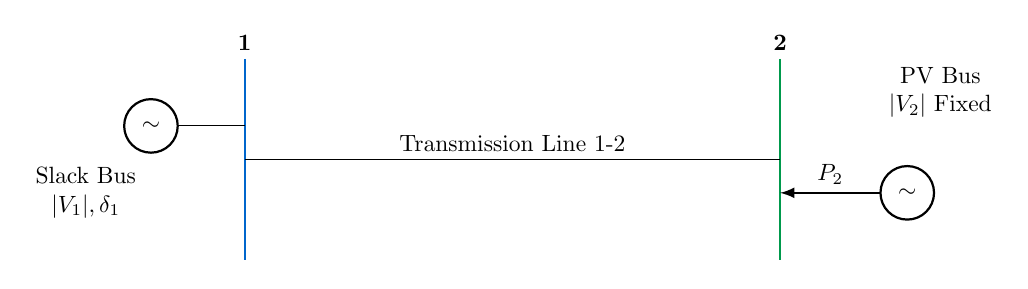
\begin{tikzpicture}[>=latex, scale=0.85, transform shape]
    % Bus 1 (Slack)
    \draw[thick, mainblue] (0,4.5) -- (0,1.5);
    \node[above] at (0,4.5) {\textbf{1}};
    \node[left, align=center] at (-1.5,2.5) {Slack Bus\\$|V_1|, \delta_1$};
    \draw (0,3.5) -- (-1,3.5);
    \draw[thick] (-1.4,3.5) circle (0.4) node {$\sim$};

    % Bus 2 (PV)
    \draw[thick, conceptgreen] (8,4.5) -- (8,1.5);
    \node[above] at (8,4.5) {\textbf{2}};
    \node[right, align=center] at (9.5,4.0) {PV Bus\\$|V_2|$ Fixed};
    \draw[->, thick] (9.5,2.5) -- (8,2.5) node[midway, above] {$P_2$}; % P gen injected
    \draw[thick] (9.9,2.5) circle (0.4) node {$\sim$};

    % Line
    \draw (0,3) -- (8,3) node[midway, above] {Transmission Line 1-2};
\end{tikzpicture}
\end{center}

\textbf{Matrix Equation for Example 1:}
\begin{equation*}
    \begin{bmatrix} 
    \Delta P_2 
    \end{bmatrix} 
    = 
    \begin{bmatrix} 
    \frac{\partial P_2}{\partial \delta_2} 
    \end{bmatrix}
    \begin{bmatrix} 
    \Delta \delta_2 
    \end{bmatrix}
\end{equation*}

\vspace{0.8cm}

% --- EXAMPLE 2 ---
\noindent \textbf{\large Example 2: 3-Bus System (1 Slack, 2 PV Buses)} \\
Here, Bus 1 is Slack, while both Bus 2 and Bus 3 are Generator (PV) buses. The only unknowns in the entire system are the voltage angles of the two generators ($\Delta \delta_2$ and $\Delta \delta_3$).
\begin{center}
\begin{tikzpicture}[>=latex, scale=0.85, transform shape]
    % Bus 1 (Slack)
    \draw[thick, mainblue] (0,4.5) -- (0,1.5);
    \node[above] at (0,4.5) {\textbf{1}};
    \node[left, align=center] at (-1.5,2.5) {Slack Bus\\$|V_1|, \delta_1$};
    \draw (0,3.5) -- (-1,3.5);
    \draw[thick] (-1.4,3.5) circle (0.4) node {$\sim$};

    % Bus 2 (PV)
    \draw[thick, conceptgreen] (10,4.5) -- (10,1.5);
    \node[above] at (10,4.5) {\textbf{2}};
    \node[right, align=center] at (11.5,4.0) {PV Bus\\$|V_2|$ Fixed};
    \draw[->, thick] (11.5,2.5) -- (10,2.5) node[midway, above] {$P_2$}; 
    \draw[thick] (11.9,2.5) circle (0.4) node {$\sim$};

    % Bus 3 (PV)
    \draw[thick, conceptgreen] (3.5,0) -- (6.5,0);
    \node[left] at (3.5,0) {\textbf{3}};
    \node[left, align=center] at (2.5,-0.5) {PV Bus\\$|V_3|$ Fixed};
    \draw[->, thick] (4.5,-1.5) -- (4.5,0) node[midway, left] {$P_3$}; 
    \draw[thick] (4.5,-1.9) circle (0.4) node {$\sim$};

    % Lines
    \draw (0,4) -- (10,4) node[midway, above] {Line 1-2};
    \draw (0,2) -- (3,2) -- (3,0);
    \node[above right] at (1.5, 2) {Line 1-3};
    \draw (10,2) -- (7,2) -- (7,0);
    \node[above left] at (8.5, 2) {Line 2-3};
\end{tikzpicture}
\end{center}

\textbf{Matrix Equation for Example 2:}
\begin{equation*}
    \begin{bmatrix} 
    \Delta P_2 \\[0.3cm]
    \Delta P_3 
    \end{bmatrix} 
    = 
    \begin{bmatrix} 
    \frac{\partial P_2}{\partial \delta_2} & \frac{\partial P_2}{\partial \delta_3} \\[0.3cm]
    \frac{\partial P_3}{\partial \delta_2} & \frac{\partial P_3}{\partial \delta_3}
    \end{bmatrix}
    \begin{bmatrix} 
    \Delta \delta_2 \\[0.3cm]
    \Delta \delta_3 
    \end{bmatrix}
\end{equation*}

\vspace{0.5cm}
\hrule
\vspace{0.5cm}





\newpage
% ==========================================
% The Full 3-Bus N-R Solution
% ==========================================
\section*{\textcolor{mainblue}{Complete Newton-Raphson Example}}

\textbf{\textcolor{conceptgreen}{Problem Statement:}}
The Figure shows a 3-bus power system. Bus 1 is the slack bus with $V_1 = 1.05 \angle 0^\circ$ pu. Bus 2 is a load bus taking 400 MW and 250 Mvar. Bus 3 is a generator (PV) bus holding $|V_3| = 1.04$ pu and generating 200 MW. Line impedances are marked on a 100 MVA base. \\
\textbf{\textcolor{conceptgreen}{Goal:}} Perform two iterations of the Newton-Raphson power flow.


\begin{center}
\begin{tikzpicture}[>=latex, scale=0.9, transform shape]
    % Bus 1
    \draw[thick, mainblue] (0,4.5) -- (0,1.5);
    \node[above] at (0,4.5) {\textbf{1}};
    \node[left, align=center] at (-1.5,2.5) {Slack Bus\\$V_1 = 1.05\angle 0^\circ$};
    \draw (0,3.5) -- (-1,3.5);
    \draw[thick] (-1.4,3.5) circle (0.4) node {$\sim$};

    % Bus 2
    \draw[thick, trapred] (10,4.5) -- (10,1.5);
    \node[above] at (10,4.5) {\textbf{2}};
    \draw[->, thick] (10,3.5) -- (11.5,3.5) node[right, align=center] {400\\MW};
    \draw[->, thick] (10,2.5) -- (11.5,2.5) node[right, align=center] {250\\Mvar};
    \draw (10.4, 2.3) -- (10.4, 2.7);

    % Bus 3
    \draw[thick, conceptgreen] (3.5,0) -- (6.5,0);
    \node[left] at (3.5,0) {\textbf{3}};
    \draw[->, thick] (4.5,0) -- (4.5,-1.5) node[below, align=center] {200\\MW};
    \draw (5.5,0) -- (5.5,-0.6);
    \draw[thick] (5.5,-1) circle (0.4) node {$\sim$};
    \node[right] at (6,-1) {$|V_3| = 1.04$};

    % Lines
    \draw (0,4) -- (10,4) node[midway, above] {$0.02 + j0.04$};
    \draw (0,2) -- (3,2) -- (3,0);
    \node[above right] at (1.5, 2) {$0.01 + j0.03$};
    \draw (10,2) -- (7,2) -- (7,0);
    \node[above left] at (8.5, 2) {$0.0125 + j0.025$};
\end{tikzpicture}
\end{center}

\definecolor{solutionorange}{RGB}{230,120,20}
\section*{\textcolor{solutionorange}{Solution:}}

\section*{Iteration 1:}
\subsection*{Step-1: Convert scheduled powers to per-unit}
Convert scheduled powers to per-unit ($S_{base} = 100$ MVA):
\begin{align*}
    P_2^{sch} &= \frac{-400}{100} = -4.0 \text{ pu} \quad & Q_2^{sch} &= \frac{-250}{100} = -2.5 \text{ pu} \\
    P_3^{sch} &= \frac{200}{100} = 2.0 \text{ pu}
\end{align*}

\subsection*{Step-2: Build the $Y_{bus}$}

Calculate line admittances ($y = 1/Z$):
\begin{align*}
    y_{12} &= \frac{1}{0.02 + j0.04} = 10 - j20 \text{ pu} \\
    y_{13} &= \frac{1}{0.01 + j0.03} = 10 - j30 \text{ pu} \\
    y_{23} &= \frac{1}{0.0125 + j0.025} = 16 - j32 \text{ pu}
\end{align*}

Build the $Y_{bus}$ (extracting $G$ and $B$ components for N-R formulas):
\begin{align*}
    Y_{11} &= y_{12} + y_{13} = 20 - j50 \\
    Y_{22} &= y_{12} + y_{23} = 26 - j52 \quad &\implies G_{22} = 26, \ B_{22} = -52 \\
    Y_{33} &= y_{13} + y_{23} = 26 - j62 \quad &\implies G_{33} = 26, \ B_{33} = -62 \\
    Y_{12} &= Y_{21} = -y_{12} = -10 + j20 \quad &\implies G_{21} = -10, \ B_{21} = 20 \\
    Y_{13} &= Y_{31} = -y_{13} = -10 + j30 \quad &\implies G_{31} = -10, \ B_{31} = 30 \\
    Y_{23} &= Y_{32} = -y_{23} = -16 + j32 \quad &\implies G_{23} = -16, \ B_{23} = 32
\end{align*}

\vspace{0.5cm}

\subsection*{Step-3: Initial Guesses}
\begin{stepbox}[{Flat Start Initial Guesses}]
Since Bus 1 and Bus 3 have fixed magnitudes, and we assume a "flat start" of $0^\circ$ (or $0$ radians) for all unknown angles, our initial starting values are:

\begin{itemize}
    \item \textbf{Bus 1 (Slack):} $V_1 = 1.05 \angle 0^\circ \quad \implies \mathbf{|V_1| = 1.05 \text{ pu}, \ \delta_1 = 0 \text{ rad}}$ (Fixed)
    \item \textbf{Bus 2 (PQ):} $V_2^{(0)} = 1.0 \angle 0^\circ \quad \implies \mathbf{|V_2|^{(0)} = 1.0 \text{ pu}, \ \delta_2^{(0)} = 0 \text{ rad}}$ (Initial Guess)
    \item \textbf{Bus 3 (PV):} $V_3^{(0)} = 1.04 \angle 0^\circ \quad \implies \mathbf{|V_3|^{(0)} = 1.04 \text{ pu}, \ \delta_3^{(0)} = 0 \text{ rad}}$ ($|V|$ is Scheduled, $\delta$ is a Guess)
\end{itemize}
\end{stepbox}


\subsection*{Step-4: Calculate Power Mismatches}

\begin{stepbox}[Expanding and Calculating Initial Powers]
\textbf{1. The Load Flow Equations} \\
From the general Load Flow equations:
\begin{align}
    P_i &= \sum_{n=1}^{N} |Y_{in} V_i V_n| \cos(\theta_{in} + \delta_n - \delta_i) \tag{1} \\
    Q_i &= -\sum_{n=1}^{N} |Y_{in} V_i V_n| \sin(\theta_{in} + \delta_n - \delta_i) \tag{2}
\end{align}

\textbf{2. Expanding for our 3-Bus System} \\
Expanding equations (1) and (2) for Bus 2 ($P_2, Q_2$) and Bus 3 ($P_3$):
\begin{align}
    P_2 =\;& |V_2||V_1||Y_{21}| \cos(\theta_{21} + \delta_1 - \delta_2) \nonumber \\
    &+ |V_2|^2|Y_{22}| \cos(\theta_{22} + \cancel{\delta_2 - \delta_2}^0) \nonumber \\
    &+ |V_2||V_3||Y_{23}| \cos(\theta_{23} + \delta_3 - \delta_2) \tag{3} \\[0.3cm]
    %
    P_3 =\;& |V_3||V_1||Y_{31}| \cos(\theta_{31} + \delta_1 - \delta_3) \nonumber \\
    &+ |V_3||V_2||Y_{32}| \cos(\theta_{32} + \delta_2 - \delta_3) \nonumber \\
    &+ |V_3|^2|Y_{33}| \cos(\theta_{33} + \cancel{\delta_3 - \delta_3}^0) \tag{4} \\[0.3cm]
    %
    Q_2 =\;& -|V_2||V_1||Y_{21}| \sin(\theta_{21} + \delta_1 - \delta_2) \nonumber \\
    &- |V_2|^2|Y_{22}| \sin(\theta_{22} + 0) \nonumber \\
    &- |V_2||V_3||Y_{23}| \sin(\theta_{23} + \delta_3 - \delta_2) \tag{5}
\end{align}

\textbf{3. Relationship between $Y$, $G$, and $B$} \\
We know that $Y_{in} = G_{in} + jB_{in}$. From polar-to-rectangular conversion:
\begin{equation*}
    \therefore G_{in} = |Y_{in}|\cos(\theta_{in}) \quad \text{and} \quad B_{in} = |Y_{in}|\sin(\theta_{in})
\end{equation*}


\textbf{4. Calculate Initial Powers (Iteration 0)} \\
For the first iteration, we use our flat start guesses where all initial angles are zero: $[\delta_1 = \delta_2 = \delta_3 = 0^\circ]$. Substituting these zeros into our expanded equations (3), (4), and (5):

\noindent \textbf{From eqn-(3):}
\begin{align*}
    P_2^{(0)} &= |V_2||V_1||Y_{21}| \cos(\theta_{21}) + |V_2|^2|Y_{22}| \cos(\theta_{22}) + |V_2||V_3||Y_{23}| \cos(\theta_{23}) \\
    &= |V_2||V_1|G_{21} + |V_2|^2 G_{22} + |V_2||V_3|G_{23} \\
    &= (1 \times 1.05)(-10) + (1)^2(26) + (1 \times 1.04)(-16) \\
    &= \mathbf{-1.14 \text{ pu}}
\end{align*}

\noindent \textbf{From eqn-(4):}
\begin{align*}
    P_3^{(0)} &= |V_3||V_1||Y_{31}| \cos(\theta_{31}) + |V_3||V_2||Y_{32}| \cos(\theta_{32}) + |V_3|^2|Y_{33}| \cos(\theta_{33}) \\
    &= |V_3||V_1|G_{31} + |V_3||V_2|G_{32} + |V_3|^2 G_{33} \\
    &= (1.04 \times 1.05)(-10) + (1.04 \times 1)(-16) + (1.04)^2(26) \\
    &= \mathbf{0.5616 \text{ pu}}
\end{align*}

\noindent \textbf{From eqn-(5):}
\begin{align*}
    Q_2^{(0)} &= -|V_2||V_1||Y_{21}| \sin(\theta_{21}) - |V_2|^2|Y_{22}| \sin(\theta_{22}) - |V_2||V_3||Y_{23}| \sin(\theta_{23}) \\
    &= -|V_2||V_1|B_{21} - |V_2|^2 B_{22} - |V_2||V_3|B_{23} \\
    &= -(1 \times 1.05)(20) - (1)^2(-52) - (1 \times 1.04)(32) \\
    &= \mathbf{-2.28 \text{ pu}}
\end{align*}

\vspace{0.3cm}
\hrule
\vspace{0.3cm}

\textbf{5. Find the Power Mismatches ($\Delta$)} \\
Finally, subtract the initial powers we just calculated from the actual scheduled powers:
\begin{align*}
    \Delta P_2 &= P_2^{sch} - P_2^{(0)} = -4.0 - (-1.14) = \mathbf{-2.86 \text{ pu}} \\
    \Delta P_3 &= P_3^{sch} - P_3^{(0)} = 2.0 - (0.5616) = \mathbf{1.4384 \text{ pu}} \\
    \Delta Q_2 &= Q_2^{sch} - Q_2^{(0)} = -2.5 - (-2.28) = \mathbf{-0.22 \text{ pu}}
\end{align*}
\end{stepbox}


\begin{conceptbox}[Why is there no $\Delta Q_3$?]
Bus 3 is a generator (PV) bus! We do not know its scheduled reactive power limit yet, so we cannot calculate a mismatch. We omit its row from the matrix entirely.
\end{conceptbox}

\subsection*{Step-5: Build the Jacobian Matrixs}
\begin{stepbox}[Build the $3 \times 3$ Jacobian Matrix (Step-by-Step Calculus)]

\textbf{1. The Jacobian Matrix Equation}\\
To solve the system, we need to populate the $3 \times 3$ Jacobian matrix ($J$) that relates our Mismatches to our Corrections:
\begin{equation*}
    \begin{bmatrix} \Delta P_2 \\ \Delta P_3 \\ \Delta Q_2 \end{bmatrix} = 
    \begin{bmatrix} 
    \frac{\partial P_2}{\partial \delta_2} & \frac{\partial P_2}{\partial \delta_3} & \frac{\partial P_2}{\partial |V_2|} \\[0.3cm]
    \frac{\partial P_3}{\partial \delta_2} & \frac{\partial P_3}{\partial \delta_3} & \frac{\partial P_3}{\partial |V_2|} \\[0.3cm]
    \frac{\partial Q_2}{\partial \delta_2} & \frac{\partial Q_2}{\partial \delta_3} & \frac{\partial Q_2}{\partial |V_2|} 
    \end{bmatrix}
    \begin{bmatrix} \Delta \delta_2 \\ \Delta \delta_3 \\ \Delta |V_2| \end{bmatrix}
\end{equation*}

\vspace{0.3cm}
\textbf{2. Calculate Partial Derivatives (Row 1: Derivatives of $P_2$)}\\
%
\noindent \textbf{Element $J_{11} \ (\partial P_2 / \partial \delta_2)$:} \\
From eqn-(3):
\begin{align*}
    P_2 =\;& |V_2||V_1||Y_{21}| \cos(\theta_{21} + \delta_1 - \delta_2) + |V_2|^2|Y_{22}| \cos(\theta_{22}) + |V_2||V_3||Y_{23}| \cos(\theta_{23} + \delta_3 - \delta_2) \\[0.2cm]
    %
    \therefore \frac{\partial P_2}{\partial \delta_2} =\;& |V_2||V_1||Y_{21}| \left\{-\sin(\theta_{21} + \delta_1 - \delta_2) \cdot (0 + 0 - 1)\right\} \\
    & + 0 \\
    & + |V_2||V_3||Y_{23}| \left\{-\sin(\theta_{23} + \delta_3 - \delta_2) \cdot (0 + 0 - 1)\right\} \\[0.2cm]
    %
    =\;& |V_2||V_1|\underbrace{|Y_{21}|\sin(\theta_{21} + 0)}_{B_{21}} + |V_2||V_3|\underbrace{|Y_{23}|\sin(\theta_{23} + 0)}_{B_{23}} \quad \text{\textcolor{mainblue}{(Apply Flat Start: $\delta=0$)}} \\[0.2cm]
    %
    =\;& |V_2||V_1|B_{21} + |V_2||V_3|B_{23} \\
    =\;& (1 \times 1.05)(20) + (1 \times 1.04)(32) \\
    =\;& \mathbf{54.28}
\end{align*}

% ================= J12 =================
\vspace{0.3cm}
\noindent \textbf{Element $J_{12} \ (\partial P_2 / \partial \delta_3)$:} \\
From eqn-(3):
\begin{align*}
    P_2 =\;& |V_2||V_1||Y_{21}| \cos(\theta_{21} + \delta_1 - \delta_2) + |V_2|^2|Y_{22}| \cos(\theta_{22}) + |V_2||V_3||Y_{23}| \cos(\theta_{23} + \delta_3 - \delta_2) \\[0.2cm]
    %
    \therefore \frac{\partial P_2}{\partial \delta_3} =\;& 0 + 0 + |V_2||V_3||Y_{23}| \left\{-\sin(\theta_{23} + \delta_3 - \delta_2) \cdot (0 + 1 - 0)\right\} \\[0.2cm]
    %
    =\;& -|V_2||V_3|\underbrace{|Y_{23}|\sin(\theta_{23} + 0)}_{B_{23}} \quad \text{\textcolor{mainblue}{(Apply Flat Start: $\delta=0$)}} \\[0.2cm]
    %
    =\;& -|V_2||V_3|B_{23} \\
    =\;& -(1 \times 1.04)(32) \\
    =\;& \mathbf{-33.28}
\end{align*}

\newpage
% ================= J13 =================
\vspace{0.3cm}
\noindent \textbf{Element $J_{13} \ (\partial P_2 / \partial |V_2|)$:} \\
From eqn-(3):
\begin{align*}
    P_2 =\;& |V_2||V_1||Y_{21}| \cos(\theta_{21} + \delta_1 - \delta_2) + |V_2|^2|Y_{22}| \cos(\theta_{22}) + |V_2||V_3||Y_{23}| \cos(\theta_{23} + \delta_3 - \delta_2) \\[0.2cm]
    %
    \therefore \frac{\partial P_2}{\partial |V_2|} =\;& |V_1||Y_{21}| \cos(\theta_{21} + \delta_1 - \delta_2) + 2|V_2||Y_{22}| \cos(\theta_{22}) + |V_3||Y_{23}| \cos(\theta_{23} + \delta_3 - \delta_2) \\[0.2cm]
    %
    =\;& |V_1|\underbrace{|Y_{21}|\cos(\theta_{21} + 0)}_{G_{21}} + 2|V_2|\underbrace{|Y_{22}|\cos(\theta_{22})}_{G_{22}} + |V_3|\underbrace{|Y_{23}|\cos(\theta_{23} + 0)}_{G_{23}} \quad \text{\textcolor{mainblue}{(Flat Start)}} \\[0.2cm]
    %
    =\;& |V_1|G_{21} + 2|V_2|G_{22} + |V_3|G_{23} \\
    =\;& (1.05)(-10) + 2(1)(26) + (1.04)(-16) \\
    =\;& \mathbf{24.86}
\end{align*}

\vspace{0.3cm}
% ================= J21 =================
\vspace{0.5cm}
\textbf{3. Calculate Partial Derivatives (Row 2: Derivatives of $P_3$)}\\
%
\noindent \textbf{Element $J_{21} \ (\partial P_3 / \partial \delta_2)$:} \\
From eqn-(4):
\begin{align*}
    P_3 =\;& |V_3||V_1||Y_{31}| \cos(\theta_{31} + \delta_1 - \delta_3) + |V_3||V_2||Y_{32}| \cos(\theta_{32} + \delta_2 - \delta_3) + |V_3|^2|Y_{33}| \cos(\theta_{33}) \\[0.2cm]
    %
    \therefore \frac{\partial P_3}{\partial \delta_2} =\;& 0 + |V_3||V_2||Y_{32}| \left\{-\sin(\theta_{32} + \delta_2 - \delta_3) \cdot (0 + 1 - 0)\right\} + 0 \\[0.2cm]
    %
    =\;& -|V_3||V_2|\underbrace{|Y_{32}|\sin(\theta_{32} + 0)}_{B_{32}} \quad \text{\textcolor{mainblue}{(Apply Flat Start: $\delta=0$)}} \\[0.2cm]
    %
    =\;& -|V_3||V_2|B_{32} \\
    =\;& -(1.04 \times 1)(32) \\
    =\;& \mathbf{-33.28}
\end{align*}

% ================= J22 =================
\vspace{0.3cm}
\noindent \textbf{Element $J_{22} \ (\partial P_3 / \partial \delta_3)$:} \\
From eqn-(4):
\begin{align*}
    P_3 =\;& |V_3||V_1||Y_{31}| \cos(\theta_{31} + \delta_1 - \delta_3) + |V_3||V_2||Y_{32}| \cos(\theta_{32} + \delta_2 - \delta_3) + |V_3|^2|Y_{33}| \cos(\theta_{33}) \\[0.2cm]
    %
    \therefore \frac{\partial P_3}{\partial \delta_3} =\;& |V_3||V_1||Y_{31}| \left\{-\sin(\theta_{31} + \delta_1 - \delta_3) \cdot (0 + 0 - 1)\right\} \\
    & + |V_3||V_2||Y_{32}| \left\{-\sin(\theta_{32} + \delta_2 - \delta_3) \cdot (0 + 0 - 1)\right\} \\
    & + 0 \\[0.2cm]
    %
    =\;& |V_3||V_1|\underbrace{|Y_{31}|\sin(\theta_{31} + 0)}_{B_{31}} + |V_3||V_2|\underbrace{|Y_{32}|\sin(\theta_{32} + 0)}_{B_{32}} \quad \text{\textcolor{mainblue}{(Apply Flat Start: $\delta=0$)}} \\[0.2cm]
    %
    =\;& |V_3||V_1|B_{31} + |V_3||V_2|B_{32} \\
    =\;& (1.04 \times 1.05)(30) + (1.04 \times 1)(32) \\
    =\;& \mathbf{66.04}
\end{align*}

\newpage
% ================= J23 =================
\vspace{0.3cm}
\noindent \textbf{Element $J_{23} \ (\partial P_3 / \partial |V_2|)$:} \\
From eqn-(4):
\begin{align*}
    P_3 =\;& |V_3||V_1||Y_{31}| \cos(\theta_{31} + \delta_1 - \delta_3) + |V_3||V_2||Y_{32}| \cos(\theta_{32} + \delta_2 - \delta_3) + |V_3|^2|Y_{33}| \cos(\theta_{33}) \\[0.2cm]
    %
    \therefore \frac{\partial P_3}{\partial |V_2|} =\;& 0 + |V_3||Y_{32}| \cos(\theta_{32} + \delta_2 - \delta_3) + 0 \\[0.2cm]
    %
    =\;& |V_3|\underbrace{|Y_{32}|\cos(\theta_{32} + 0)}_{G_{32}} \quad \text{\textcolor{mainblue}{(Apply Flat Start: $\delta=0$)}} \\[0.2cm]
    %
    =\;& |V_3|G_{32} \\
    =\;& (1.04)(-16) \\
    =\;& \mathbf{-16.64}
\end{align*}

\vspace{0.3cm}
% ================= J31 =================
\vspace{0.5cm}
\textbf{4. Calculate Partial Derivatives (Row 3: Derivatives of $Q_2$)}\\
%
\noindent \textbf{Element $J_{31} \ (\partial Q_2 / \partial \delta_2)$:} \\
From eqn-(5):
\begin{align*}
    Q_2 =\;& -|V_2||V_1||Y_{21}| \sin(\theta_{21} + \delta_1 - \delta_2) - |V_2|^2|Y_{22}| \sin(\theta_{22}) - |V_2||V_3||Y_{23}| \sin(\theta_{23} + \delta_3 - \delta_2) \\[0.2cm]
    %
    \therefore \frac{\partial Q_2}{\partial \delta_2} =\;& -|V_2||V_1||Y_{21}| \left\{\cos(\theta_{21} + \delta_1 - \delta_2) \cdot (0 + 0 - 1)\right\} \\
    & - 0 \\
    & - |V_2||V_3||Y_{23}| \left\{\cos(\theta_{23} + \delta_3 - \delta_2) \cdot (0 + 0 - 1)\right\} \\[0.2cm]
    %
    =\;& |V_2||V_1|\underbrace{|Y_{21}|\cos(\theta_{21} + 0)}_{G_{21}} + |V_2||V_3|\underbrace{|Y_{23}|\cos(\theta_{23} + 0)}_{G_{23}} \quad \text{\textcolor{mainblue}{(Apply Flat Start: $\delta=0$)}} \\[0.2cm]
    %
    =\;& |V_2||V_1|G_{21} + |V_2||V_3|G_{23} \\
    =\;& (1 \times 1.05)(-10) + (1 \times 1.04)(-16) \\
    =\;& \mathbf{-27.14}
\end{align*}

% ================= J32 =================
\vspace{0.3cm}
\noindent \textbf{Element $J_{32} \ (\partial Q_2 / \partial \delta_3)$:} \\
From eqn-(5):
\begin{align*}
    Q_2 =\;& -|V_2||V_1||Y_{21}| \sin(\theta_{21} + \delta_1 - \delta_2) - |V_2|^2|Y_{22}| \sin(\theta_{22}) - |V_2||V_3||Y_{23}| \sin(\theta_{23} + \delta_3 - \delta_2) \\[0.2cm]
    %
    \therefore \frac{\partial Q_2}{\partial \delta_3} =\;& 0 - 0 - |V_2||V_3||Y_{23}| \left\{\cos(\theta_{23} + \delta_3 - \delta_2) \cdot (0 + 1 - 0)\right\} \\[0.2cm]
    %
    =\;& -|V_2||V_3|\underbrace{|Y_{23}|\cos(\theta_{23} + 0)}_{G_{23}} \quad \text{\textcolor{mainblue}{(Apply Flat Start: $\delta=0$)}} \\[0.2cm]
    %
    =\;& -|V_2||V_3|G_{23} \\
    =\;& -(1 \times 1.04)(-16) \\
    =\;& \mathbf{16.64}
\end{align*}

\newpage
% ================= J33 =================
\vspace{0.3cm}
\noindent \textbf{Element $J_{33} \ (\partial Q_2 / \partial |V_2|)$:} \\
From eqn-(5):
\begin{align*}
    Q_2 =\;& -|V_2||V_1||Y_{21}| \sin(\theta_{21} + \delta_1 - \delta_2) - |V_2|^2|Y_{22}| \sin(\theta_{22}) - |V_2||V_3||Y_{23}| \sin(\theta_{23} + \delta_3 - \delta_2) \\[0.2cm]
    %
    \therefore \frac{\partial Q_2}{\partial |V_2|} =\;& -|V_1||Y_{21}| \sin(\theta_{21} + \delta_1 - \delta_2) - 2|V_2||Y_{22}| \sin(\theta_{22}) - |V_3||Y_{23}| \sin(\theta_{23} + \delta_3 - \delta_2) \\[0.2cm]
    %
    =\;& -|V_1|\underbrace{|Y_{21}|\sin(\theta_{21} + 0)}_{B_{21}} - 2|V_2|\underbrace{|Y_{22}|\sin(\theta_{22})}_{B_{22}} - |V_3|\underbrace{|Y_{23}|\sin(\theta_{23} + 0)}_{B_{23}} \quad \text{\textcolor{mainblue}{(Flat Start)}} \\[0.2cm]
    %
    =\;& -|V_1|B_{21} - 2|V_2|B_{22} - |V_3|B_{23} \\
    =\;& -(1.05)(20) - 2(1)(-52) - (1.04)(32) \\
    =\;& \mathbf{49.72}
\end{align*}
\end{stepbox}


\subsection*{Step-6: Matrix Inversion \& Voltage Update}
\begin{stepbox}[{Matrix Inversion \& Voltage Update}]
First, we write the general Newton-Raphson matrix equation for our 3-bus system:
\begin{equation*}
    \begin{bmatrix} \Delta P_2 \\ \Delta P_3 \\ \Delta Q_2 \end{bmatrix} 
    = 
    \begin{bmatrix} 
    J_{11} & J_{12} & J_{13} \\ 
    J_{21} & J_{22} & J_{23} \\ 
    J_{31} & J_{32} & J_{33} 
    \end{bmatrix} 
    \begin{bmatrix} \Delta \delta_2 \\ \Delta \delta_3 \\ \Delta |V_2| \end{bmatrix}
\end{equation*}

Now, substituting the calculated power mismatches and Jacobian elements into the equation:
\begin{equation*}
    \begin{bmatrix} -2.86 \\ 1.4384 \\ -0.22 \end{bmatrix} 
    = 
    \begin{bmatrix} 
    54.28 & -33.28 & 24.86 \\ 
    -33.28 & 66.04 & -16.64 \\ 
    -27.14 & 16.64 & 49.72 
    \end{bmatrix} 
    \begin{bmatrix} \Delta \delta_2 \\ \Delta \delta_3 \\ \Delta |V_2| \end{bmatrix}
\end{equation*}

Solving this linear system (via matrix inversion on a calculator) yields the voltage corrections:
\begin{align*}
    \Delta \delta_2 &= \mathbf{-0.04526 \text{ rad}} \\
    \Delta \delta_3 &= \mathbf{-0.00772 \text{ rad}} \\
    \Delta |V_2| &= \mathbf{-0.02655 \text{ pu}}
\end{align*}

\textbf{Final Updated Voltages for Iteration 1:}
\begin{align*}
    |V_2|^{(1)} &= |V_2|^{(0)} + \Delta |V_2| = 1.0 + (-0.02655) = \mathbf{0.97345 \text{ pu}} \\
    \delta_2^{(1)} &= \delta_2^{(0)} + \Delta \delta_2 = 0 + (-0.04526 \text{ rad}) \times \frac{180^\circ}{\pi} = \mathbf{-2.593^\circ} \\
    \delta_3^{(1)} &= \delta_3^{(0)} + \Delta \delta_3 = 0 + (-0.00772 \text{ rad}) \times \frac{180^\circ}{\pi} = \mathbf{-0.442^\circ}
\end{align*}
\vspace{0.3cm}
\textbf{Final Answer (End of Iteration 1):} \\
Bus 2 Voltage: $V_2^{(1)} = 0.97345 \angle -2.593^\circ \text{ pu}$ \\
Bus 3 Voltage: $V_3^{(1)} = 1.04 \angle -0.442^\circ \text{ pu}$
\end{stepbox}



\newpage
% ==========================================
% ITERATION 2
% ==========================================
\section*{Iteration 2 Execution}

\begin{stepbox}[Step 1: The New Starting Values]
We begin Iteration 2 using the updated voltages we just found at the end of Iteration 1. 
\textbf{Crucial Note:} All angles MUST be in radians for the calculus to work!
\begin{align*}
    V_1 &= 1.05 \angle 0 \text{ rad (Fixed)} \\
    |V_2|^{(1)} &= 0.97345 \text{ pu}, \quad \delta_2^{(1)} = -0.045263 \text{ rad} \\
    |V_3|^{(1)} &= 1.04 \text{ pu}, \quad \delta_3^{(1)} = -0.007718 \text{ rad}
\end{align*}
\end{stepbox}

\begin{stepbox}[Step 2: Pre-calculate Polar Admittances \& Angles]
Because the voltage angles ($\delta$) are no longer zero, we cannot use the simple $G$ and $B$ shortcut anymore. We must use the full trigonometric equations. To make our math cleaner, we will first convert our required $Y_{bus}$ elements to Polar form ($|Y| \angle \theta$) and pre-calculate the repeating angle arguments.

\textbf{1. Convert $Y_{bus}$ to Polar Form (in Radians):}\\
We convert rectangular elements ($G + jB$) into magnitude $|Y| = \sqrt{G^2 + B^2}$ and angle $\theta = \tan^{-1}(B/G)$. \textit{(*Remember to add $\pi$ if the real part $G$ is negative!)}
\begin{align*}
    Y_{21} &= -10 + j20 \implies |Y_{21}| = \mathbf{22.36068}, \quad \theta_{21} = \tan^{-1}\left(\frac{20}{-10}\right) + \pi = \mathbf{2.0344 \text{ rad}} \\[0.2cm]
    Y_{22} &= 26 - j52 \implies |Y_{22}| = \mathbf{58.13777}, \quad \theta_{22} = \tan^{-1}\left(\frac{-52}{26}\right) = \mathbf{-1.1071 \text{ rad}} \\[0.2cm]
    Y_{23} &= -16 + j32 \implies |Y_{23}| = \mathbf{35.77709}, \quad \theta_{23} = \tan^{-1}\left(\frac{32}{-16}\right) + \pi = \mathbf{2.0344 \text{ rad}} \\[0.2cm]
    Y_{31} &= -10 + j30 \implies |Y_{31}| = \mathbf{31.62278}, \quad \theta_{31} = \tan^{-1}\left(\frac{30}{-10}\right) + \pi = \mathbf{1.8925 \text{ rad}} \\[0.2cm]
    Y_{32} &= -16 + j32 \implies |Y_{32}| = \mathbf{35.77709}, \quad \theta_{32} = \tan^{-1}\left(\frac{32}{-16}\right) + \pi = \mathbf{2.0344 \text{ rad}} \\[0.2cm]
    Y_{33} &= 26 - j62 \implies |Y_{33}| = \mathbf{67.23094}, \quad \theta_{33} = \tan^{-1}\left(\frac{-62}{26}\right) = \mathbf{-1.1733 \text{ rad}}
\end{align*}

\textbf{2. Pre-calculate the Angle Arguments ($\alpha$):}\\
To save massive amounts of space in our equations, let's calculate the repeating angle combinations $\alpha_{ij} = (\theta_{ij} - \delta_i + \delta_j)$ using our current Iteration 1 angles:
\begin{align*}
    \alpha_{21} &= \theta_{21} - \delta_2 + \delta_1 = 2.0344 - (-0.045263) + 0 = \mathbf{2.079663 \text{ rad}} \\
    \alpha_{23} &= \theta_{23} - \delta_2 + \delta_3 = 2.0344 - (-0.045263) + (-0.007718) = \mathbf{2.071945 \text{ rad}} \\
    \alpha_{31} &= \theta_{31} - \delta_3 + \delta_1 = 1.8925 - (-0.007718) + 0 = \mathbf{1.900218 \text{ rad}} \\
    \alpha_{32} &= \theta_{32} - \delta_3 + \delta_2 = 2.0344 - (-0.007718) + (-0.045263) = \mathbf{1.996855 \text{ rad}}
\end{align*}
\end{stepbox}

\newpage
\begin{examtrap}[The Quadrant Trap: Converting $Y_{bus}$ to Polar]
When converting the rectangular $Y_{bus}$ elements ($G + jB$) to polar angles ($\theta$), you must be careful with your calculator's $\tan^{-1}(B/G)$ function!

For element $Y_{21} = -10 + j20$:
\begin{itemize}
    \item The Real part ($G$) is negative, and the Imaginary part ($B$) is positive. This vector lives in the \textbf{2nd Quadrant}.
    \item A calculator will read $\tan^{-1}(20/-10)$ as $\tan^{-1}(-2)$ and give you $-63.43^\circ$ (4th Quadrant). This is mathematically incorrect for our vector!
    \item \textbf{The Rule:} If the Real part ($G$) is negative, you MUST add $180^\circ$ (or $\pi$ radians) to the calculator's answer.
\end{itemize}
$$ \theta_{21} = -63.43^\circ + 180^\circ = 116.56^\circ $$
$$ \theta_{21} \text{ (in radians)} = 116.56^\circ \times \left( \frac{\pi}{180} \right) = \mathbf{2.0344 \text{ rad}} $$
Always double-check your signs before finalizing your polar $Y_{bus}$ matrix!
\end{examtrap}

\begin{stepbox}[Step 3: Calculate New Power Mismatche]
Now we plug our Iteration 1 voltages and our pre-calculated $\alpha$ angles into the full trigonometric power equations to find our calculated powers, and then subtract them from the scheduled values.

\textbf{1. Calculate Real Power Mismatch at Bus 2 ($\Delta P_2^{(1)}$):}
\begin{align*}
    P_2^{(1)} &= |V_2||V_1||Y_{21}|\cos(\alpha_{21}) + |V_2|^2|Y_{22}|\cos(\theta_{22}) + |V_2||V_3||Y_{23}|\cos(\alpha_{23}) \\[0.2cm]
    &= (0.97345)(1.05)(22.36068)\cos(2.079663) \\
    &\quad + (0.97345)^2(58.13777)\cos(-1.1071) \\
    &\quad + (0.97345)(1.04)(35.77709)\cos(2.071945) \\[0.2cm]
    &= (-11.135) + (24.639) + (-17.405) = \mathbf{-3.900782 \text{ pu}} \\[0.3cm]
    %
    \implies \Delta P_2^{(1)} &= P_2^{sch} - P_2^{(1)} = -4.0 - (-3.900782) = \mathbf{-0.099218 \text{ pu}}
\end{align*}

\textbf{2. Calculate Real Power Mismatch at Bus 3 ($\Delta P_3^{(1)}$):}
\begin{align*}
    P_3^{(1)} &= |V_3||V_1||Y_{31}|\cos(\alpha_{31}) + |V_3||V_2||Y_{32}|\cos(\alpha_{32}) + |V_3|^2|Y_{33}|\cos(\theta_{33}) \\[0.2cm]
    &= (1.04)(1.05)(31.62278)\cos(1.900218) \\
    &\quad + (1.04)(0.97345)(35.77709)\cos(1.996855) \\
    &\quad + (1.04)^2(67.23094)\cos(-1.1733) \\[0.2cm]
    &= (-11.167) + (-14.975) + (28.120) = \mathbf{1.978285 \text{ pu}} \\[0.3cm]
    %
    \implies \Delta P_3^{(1)} &= P_3^{sch} - P_3^{(1)} = 2.0 - (1.978285) = \mathbf{0.021715 \text{ pu}}
\end{align*}

\textbf{3. Calculate Reactive Power Mismatch at Bus 2 ($\Delta Q_2^{(1)}$):}
\begin{align*}
    Q_2^{(1)} &= -|V_2||V_1||Y_{21}|\sin(\alpha_{21}) - |V_2|^2|Y_{22}|\sin(\theta_{22}) - |V_2||V_3||Y_{23}|\sin(\alpha_{23}) \\[0.2cm]
    &= -(0.97345)(1.05)(22.36068)\sin(2.079663) \\
    &\quad - (0.97345)^2(58.13777)\sin(-1.1071) \\
    &\quad - (0.97345)(1.04)(35.77709)\sin(2.071945) \\[0.2cm]
    &= -(19.962) - (-49.271) - (31.758) = \mathbf{-2.449086 \text{ pu}} \\[0.3cm]
    %
    \implies \Delta Q_2^{(1)} &= Q_2^{sch} - Q_2^{(1)} = -2.5 - (-2.449086) = \mathbf{-0.050914 \text{ pu}}
\end{align*}
\end{stepbox}

\begin{stepbox}[Step 4: Evaluate the New Jacobian Matrix (Step-by-Step)]
Because we already pre-calculated our polar $Y_{bus}$ elements and our argument angles ($\alpha_{ij}$) in Step 2, evaluating the Jacobian is simply a matter of taking the partial derivatives and plugging those pre-calculated values in!

\vspace{0.3cm}
\textbf{1. Calculate Partial Derivatives (Row 1: Derivatives of $P_2$)}\\
%
\noindent \textbf{Element $J_{11} \ (\partial P_2 / \partial \delta_2)$:} \\
From the $P_2$ equation:
\begin{align*}
    P_2 =\;& |V_2||V_1||Y_{21}| \cos(\theta_{21} + \delta_1 - \delta_2) + |V_2|^2|Y_{22}| \cos(\theta_{22}) + |V_2||V_3||Y_{23}| \cos(\theta_{23} + \delta_3 - \delta_2) \\[0.2cm]
    %
    \therefore \frac{\partial P_2}{\partial \delta_2} =\;& |V_2||V_1||Y_{21}| \left\{-\sin(\theta_{21} + \delta_1 - \delta_2) \cdot (-1)\right\} \\
    & + 0 \\
    & + |V_2||V_3||Y_{23}| \left\{-\sin(\theta_{23} + \delta_3 - \delta_2) \cdot (-1)\right\} \\[0.2cm]
    %
    =\;& |V_2||V_1||Y_{21}|\sin(\underbrace{\theta_{21} + \delta_1 - \delta_2}_{\alpha_{21}}) + |V_2||V_3||Y_{23}|\sin(\underbrace{\theta_{23} + \delta_3 - \delta_2}_{\alpha_{23}}) \\[0.2cm]
    %
    =\;& |V_2||V_1||Y_{21}|\sin(\alpha_{21}) + |V_2||V_3||Y_{23}|\sin(\alpha_{23}) \\
    =\;& (0.97345)(1.05)(22.36068)\sin(2.079663) + (0.97345)(1.04)(35.77709)\sin(2.071945) \\
    =\;& 19.9272 + 31.7974 = \mathbf{51.724675}
\end{align*}

\vspace{0.3cm}
\noindent \textbf{Element $J_{12} \ (\partial P_2 / \partial \delta_3)$:} \\
\begin{align*}
    \frac{\partial P_2}{\partial \delta_3} =\;& 0 + 0 + |V_2||V_3||Y_{23}| \left\{-\sin(\theta_{23} + \delta_3 - \delta_2) \cdot (1)\right\} \\[0.2cm]
    %
    =\;& -|V_2||V_3||Y_{23}|\sin(\alpha_{23}) \\
    =\;& -(0.97345)(1.04)(35.77709)\sin(2.071945) \\
    =\;& \mathbf{-31.765618}
\end{align*}

\vspace{0.3cm}
\noindent \textbf{Element $J_{13} \ (\partial P_2 / \partial |V_2|)$:} \\
\begin{align*}
    \frac{\partial P_2}{\partial |V_2|} =\;& |V_1||Y_{21}| \cos(\theta_{21} + \delta_1 - \delta_2) + 2|V_2||Y_{22}| \cos(\theta_{22}) + |V_3||Y_{23}| \cos(\theta_{23} + \delta_3 - \delta_2) \\[0.2cm]
    %
    =\;& |V_1||Y_{21}|\cos(\alpha_{21}) + 2|V_2||Y_{22}|\cos(\theta_{22}) + |V_3||Y_{23}|\cos(\alpha_{23}) \\
    =\;& (1.05)(22.36068)\cos(2.079663) + 2(0.97345)(58.13777)\cos(-1.1071) \\
    & + (1.04)(35.77709)\cos(2.071945) \\
    =\;& -11.5165 + 50.6062 - 17.7871 = \mathbf{21.302567}
\end{align*}

\vspace{0.5cm}
\textbf{2. Calculate Partial Derivatives (Row 2: Derivatives of $P_3$)}\\
%
\noindent \textbf{Element $J_{21} \ (\partial P_3 / \partial \delta_2)$:} \\
From the $P_3$ equation:
\begin{align*}
    P_3 =\;& |V_3||V_1||Y_{31}| \cos(\theta_{31} + \delta_1 - \delta_3) + |V_3||V_2||Y_{32}| \cos(\theta_{32} + \delta_2 - \delta_3) + |V_3|^2|Y_{33}| \cos(\theta_{33}) \\[0.2cm]
    %
    \therefore \frac{\partial P_3}{\partial \delta_2} =\;& 0 + |V_3||V_2||Y_{32}| \left\{-\sin(\theta_{32} + \delta_2 - \delta_3) \cdot (1)\right\} + 0 \\[0.2cm]
    %
    =\;& -|V_3||V_2||Y_{32}|\sin(\alpha_{32}) \\
    =\;& -(1.04)(0.97345)(35.77709)\sin(1.996855) \\
    =\;& \mathbf{-32.981642}
\end{align*}

\vspace{0.3cm}
\noindent \textbf{Element $J_{22} \ (\partial P_3 / \partial \delta_3)$:} \\
\begin{align*}
    \frac{\partial P_3}{\partial \delta_3} =\;& |V_3||V_1||Y_{31}| \left\{-\sin(\theta_{31} + \delta_1 - \delta_3) \cdot (-1)\right\} \\
    & + |V_3||V_2||Y_{32}| \left\{-\sin(\theta_{32} + \delta_2 - \delta_3) \cdot (-1)\right\} + 0 \\[0.2cm]
    %
    =\;& |V_3||V_1||Y_{31}|\sin(\alpha_{31}) + |V_3||V_2||Y_{32}|\sin(\alpha_{32}) \\
    =\;& (1.04)(1.05)(31.62278)\sin(1.900218) + (1.04)(0.97345)(35.77709)\sin(1.996855) \\
    =\;& 32.6747 + 32.9816 = \mathbf{65.656383}
\end{align*}

\vspace{0.3cm}
\noindent \textbf{Element $J_{23} \ (\partial P_3 / \partial |V_2|)$:} \\
\begin{align*}
    \frac{\partial P_3}{\partial |V_2|} =\;& 0 + |V_3||Y_{32}| \cos(\theta_{32} + \delta_2 - \delta_3) + 0 \\[0.2cm]
    %
    =\;& |V_3||Y_{32}|\cos(\alpha_{32}) \\
    =\;& (1.04)(35.77709)\cos(1.996855) \\
    =\;& \mathbf{-15.379086}
\end{align*}

\vspace{0.5cm}
\textbf{3. Calculate Partial Derivatives (Row 3: Derivatives of $Q_2$)}\\
%
\noindent \textbf{Element $J_{31} \ (\partial Q_2 / \partial \delta_2)$:} \\
From the $Q_2$ equation:
\begin{align*}
    Q_2 =\;& -|V_2||V_1||Y_{21}| \sin(\theta_{21} + \delta_1 - \delta_2) - |V_2|^2|Y_{22}| \sin(\theta_{22}) - |V_2||V_3||Y_{23}| \sin(\theta_{23} + \delta_3 - \delta_2) \\[0.2cm]
    %
    \therefore \frac{\partial Q_2}{\partial \delta_2} =\;& -|V_2||V_1||Y_{21}| \left\{\cos(\theta_{21} + \delta_1 - \delta_2) \cdot (-1)\right\} \\
    & - 0 \\
    & - |V_2||V_3||Y_{23}| \left\{\cos(\theta_{23} + \delta_3 - \delta_2) \cdot (-1)\right\} \\[0.2cm]
    %
    =\;& |V_2||V_1||Y_{21}|\cos(\alpha_{21}) + |V_2||V_3||Y_{23}|\cos(\alpha_{23}) \\
    =\;& (0.97345)(1.05)(22.36068)\cos(2.079663) + (0.97345)(1.04)(35.77709)\cos(2.071945) \\
    =\;& -11.1895 - 17.3490 = \mathbf{-28.538577}
\end{align*}

\vspace{0.3cm}
\noindent \textbf{Element $J_{32} \ (\partial Q_2 / \partial \delta_3)$:} \\
\begin{align*}
    \frac{\partial Q_2}{\partial \delta_3} =\;& 0 - 0 - |V_2||V_3||Y_{23}| \left\{\cos(\theta_{23} + \delta_3 - \delta_2) \cdot (1)\right\} \\[0.2cm]
    %
    =\;& -|V_2||V_3||Y_{23}|\cos(\alpha_{23}) \\
    =\;& -(0.97345)(1.04)(35.77709)\cos(2.071945) \\
    =\;& \mathbf{17.402838}
\end{align*}

\vspace{0.3cm}
\noindent \textbf{Element $J_{33} \ (\partial Q_2 / \partial |V_2|)$:} \\
\begin{align*}
    \frac{\partial Q_2}{\partial |V_2|} =\;& -|V_1||Y_{21}| \sin(\theta_{21} + \delta_1 - \delta_2) - 2|V_2||Y_{22}| \sin(\theta_{22}) - |V_3||Y_{23}| \sin(\theta_{23} + \delta_3 - \delta_2) \\[0.2cm]
    %
    =\;& -|V_1||Y_{21}|\sin(\alpha_{21}) - 2|V_2||Y_{22}|\sin(\theta_{22}) - |V_3||Y_{23}|\sin(\alpha_{23}) \\
    =\;& -(1.05)(22.36068)\sin(2.079663) - 2(0.97345)(58.13777)\sin(-1.1071) \\
    & - (1.04)(35.77709)\sin(2.071945) \\
    =\;& -20.4705 + 101.2173 - 32.6432 = \mathbf{48.103589}
\end{align*}

We have successfully rebuilt the Jacobian matrix for Iteration 2:
\begin{equation*}
    J^{(1)} = 
    \begin{bmatrix} 
    51.724675 & -31.765618 & 21.302567 \\ 
    -32.981642 & 65.656383 & -15.379086 \\ 
    -28.538577 & 17.402838 & 48.103589 
    \end{bmatrix}
\end{equation*}
\end{stepbox}


\begin{stepbox}[Step 5: Matrix Inversion \& Voltage Update]
We set up our Newton-Raphson system for Iteration 2 using our newly calculated mismatches and Jacobian:
\begin{equation*}
\begin{bmatrix} -0.099218 \\ 0.021715 \\ -0.050914 \end{bmatrix} 
= 
\begin{bmatrix} 
51.724675 & -31.765618 & 21.302567 \\ 
-32.981642 & 65.656383 & -15.379086 \\ 
-28.538577 & 17.402838 & 48.103589 
\end{bmatrix} 
\begin{bmatrix} \Delta \delta_2^{(1)} \\ \Delta \delta_3^{(1)} \\ \Delta |V_2|^{(1)} \end{bmatrix}
\end{equation*}

Solving this linear system gives us the new corrections:
\begin{align*}
    \Delta \delta_2^{(1)} &= \mathbf{-0.001795 \text{ rad}} \\
    \Delta \delta_3^{(1)} &= \mathbf{-0.000985 \text{ rad}} \\
    \Delta |V_2|^{(1)} &= \mathbf{-0.001767 \text{ pu}}
\end{align*}

Finally, we apply these corrections to the voltages from the end of Iteration 1 to get our Iteration 2 voltages:
\begin{align*}
    \delta_2^{(2)} &= \delta_2^{(1)} + \Delta \delta_2^{(1)} = -0.045263 + (-0.001795) = \mathbf{-0.047058 \text{ rad}} \\
    \delta_3^{(2)} &= \delta_3^{(1)} + \Delta \delta_3^{(1)} = -0.007718 + (-0.000985) = \mathbf{-0.008703 \text{ rad}} \\
    |V_2|^{(2)} &= |V_2|^{(1)} + \Delta |V_2|^{(1)} = 0.973451 + (-0.001767) = \mathbf{0.971684 \text{ pu}}
\end{align*}

\textbf{Final Answer after 2 Iterations:}\\
Bus 2 Voltage: $V_2^{(2)} = 0.971684 \angle -2.696^\circ \text{ pu}$ \\
Bus 3 Voltage: $V_3^{(2)} = 1.04 \angle -0.499^\circ \text{ pu}$

\vspace{0.3cm}
\hrule
\vspace{0.3cm}
\textit{Note: The process repeats exactly like this for Iteration 3. In the textbook, by the end of Iteration 3, the mismatches shrink to less than $0.0002$, which means the solution has fully converged!}
\end{stepbox}


\end{document}
